\subsection{FILTRATION OF THE ENVELOPING ALGEBRA}

Let g be a Lie algebra over K and T the tensor algebra of the K-module g. Let \(T^{n}\) be the submodule of T consisting of the homogeneous tensors of order n

and \(\mathrm{T_n} = \sum_{i\leqslant n}\mathrm{T^i}\) . Then \(\mathrm{T_n}\subset \mathrm{T}_{n + 1},\mathrm{T_0} = \mathrm{K}.1,\mathrm{T}_{-1} = \{0\}\) and \(\mathrm{T_nT_p}\subset \mathrm{T}_{n + p}\) . Let \(\mathbf{U}_n\) be the canonical image of \(\mathbf{T}_n\) in the enveloping algebra U of g. Then \(\mathrm{U_n}\subset \mathrm{U}_{n + 1},\mathrm{U_0} = \mathrm{K}.1,\mathrm{U}_{-1} = \{0\}\) and \(\mathrm{U_nU_p}\subset \mathrm{U}_{n + p}\) ; hence U can be described as an algebra filtered by the \(\mathbf{U}_n\) (Commutative Algebra, Chapter III, §2, no. I); the elements of \(\mathrm{U_n}\) will be said to be of filtration \(\leqslant n\) .

Let \(G^n\) be the K-module \(U_n / U_{n-1}\) and let G be the K-module the direct sum of the \(G^n\) . Multiplication on U defines, on taking quotients, a bilinear mapping of \(G^n \times G^m\) into \(G^{n+m}\) and hence a bilinear mapping of \(G \times G\) into G, which is associative. Thus G is given an associative K-algebra structure. Then \(G^n G^m \subset G^{n+m}\) . The elements of \(G^n\) are said to be of degree n.~The graded algebra thus obtained is just the graded algebra associated with the filtered algebra U (Commutative Algebra, Chapter III, § 2, no. 3).

Let \(\phi_{n}\) be the composition of the canonical K-linear mappings

\[
\mathrm{T} ^ {n} \rightarrow \mathrm{U} _ {n} \rightarrow \mathrm{G} ^ {n}.
\]

As \(\mathbf{T}^n\) is supplementary to \(\mathbf{T}_{n - 1}\) in \(\mathbf{T}_n\) , \(\phi_n\) is surjective. The \(\phi_n\) define a K-linear mapping \(\phi\) of \(\sum_{n}\mathbf{T}^{n} = \mathbf{T}\) onto \(\sum_{n}\mathbf{G}^{n} = \mathbf{G}\) .

PROPOSITION 5. The mapping \(\phi\) of T onto G is an algebra homomorphism mapping 1 to 1 and is zero on the two-sided ideal generated by the tensors \(x \otimes y - y \otimes x\) ( \(x \in \mathfrak{g}, y \in \mathfrak{g}\) ).

If \(t \in \mathbf{T}^n\) and \(t' \in \mathbf{T}^p\) , then \(\phi(t)\phi(t') = \phi(tt')\) by definition of the multiplication on \(\mathbf{G}\) . Hence \(\phi\) is an algebra homomorphism and clearly \(\phi(1) = 1\) . If \(x, y\) are in \(\mathfrak{g}\) , then \(x \otimes y - y \otimes x \in \mathbf{T}^2\) and the canonical image of this element in \(\mathrm{U}_2\) is equal to that of \([x, y]\) and therefore belongs to \(\mathrm{U}_1\) . Hence \(\phi(x \otimes y - y \otimes x) = 0\) , which proves the proposition.

Let S be the symmetric algebra of the K-module g and \(\tau\) the canonical homomorphism of T onto S. Proposition 5 proves that there exists a unique homomorphism \(\omega\) , called canonical, of the algebra S onto the algebra G, mapping 1 to 1, such that \(\phi = \omega \circ \tau\) . We have \(\omega(\mathrm{S}^{n}) = \phi(\mathrm{T}^{n}) = \mathrm{G}^{n}\) . Let \(\tau_{n}\) be the restriction of \(\tau\) to \(T^{n}\) , \(\omega_{n}\) the restriction of \(\omega\) to \(S^{n}\) , \(\psi_{n}\) the canonical mapping of \(T^{n}\) into \(U_{n}\) and \(\theta_{n}\) the canonical mapping of \(U_{n}\) onto \(G^{n}\) . The definition of \(\omega_{n}\) proves that the following diagram is commutative:

\pandocbounded{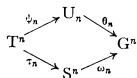
\includegraphics[keepaspectratio]{images/part001_82008693.jpg}}

PROPOSITION 6. If K is Noetherian and g is a finitely generated module, the ring U is right and left Noetherian.

S is a finitely generated algebra over K and hence a Noetherian ring (Commutative Algebra, Chapter III, § 2, no. 10, Corollary 3 to Theorem 2). Hence G, which is isomorphic to a quotient ring of S, is Noetherian. Hence U is right and left Noetherian (Commutative Algebra, Chapter III, § 2, no. 10, Remark 2).

COROLLARY. Suppose that K is a field and that g is finite-dimensional over K. Let \(I_{1}, \ldots, I_{m}\) be right (resp. left) ideals of finite codimension in U. Then the product ideal \(I_{1}I_{2}\ldots I_{m}\) is of finite codimension.

By induction on m it suffices to consider the case of, for example, two right ideals. The right U-module \(I_{1}\) is generated by a finite number of elements \(u_{1},\ldots,u_{p}\) (Proposition 6). Let \(v_{1},\ldots,v_{q}\) be elements of U whose classes modulo \(I_{2}\) generate the vector space \(U/I_{2}\) . Then the canonical images in \(I_{1}/I_{1}I_{2}\) of the \(u_{i}v_{j}\) generate the vector space \(I_{1}/I_{1}I_{2}\) , which is therefore finite-dimensional. Hence \(\dim_{\mathbb{K}}(\mathrm{U}/\mathrm{I}_{1}\mathrm{I}_{2})=\dim_{\mathbb{K}}(\mathrm{U}/\mathrm{I}_{1})+\dim_{\mathbb{K}}(\mathrm{I}_{1}/\mathrm{I}_{1}\mathrm{I}_{2})<+\infty\) .

Remark. Let \(g'\) be another Lie algebra over the ring K, \(U'\) its enveloping algebra, \(U_n'\) the set of elements of \(U'\) of filtration \(\leqslant n\) and \(U^n\) (resp. \(U'^n\) ) the set of canonical images in U (resp. \(U'\) ) of the homogeneous symmetric tensors of g (resp. \(g'\) ) of order n.~Let \(\eta\) be a homomorphism of g into \(g'\) and let \(\tilde{\eta}\) be the corresponding homomorphism of U into \(U'\) . Then

\[
\tilde {\eta} (\mathrm{U} _ {n}) \subset \mathrm{U} _ {n} ^ {\prime}, \quad \tilde {\eta} (\mathrm{U} ^ {n}) \subset \mathrm{U} ^ {\prime n}.
\]

In particular, the principal antiautomorphism of U leaves \(U_{n}\) and \(U^{n}\) stable. The K-linear mapping of \(T^{n}\) onto itself which maps

\[
x _ {1} \otimes x _ {2} \otimes \dots \otimes x _ {n} \quad \text { to } \quad x _ {n} \otimes x _ {n - 1} \otimes \dots \otimes x _ {1}
\]

for all \(x_{1},\ldots,x_{n}\) in g is a symmetry operator and hence leaves fixed the homogeneous symmetric tensors of order n.~Hence the principal antiautomorphism of U induces on each \(U^{n}\) the homothety of ratio \((-1)^{n}\) .

